% ------------------------------------------------------------------
\renewcommand{\thisweek}{MATH327 Week 5}
\renewcommand{\moddate}{Last modified 3 Mar.~2021}
\setcounter{section}{5}
\setcounter{subsection}{0}
\phantomsection
\addcontentsline{toc}{section}{Week 5: Thermodynamic cycles}
\section*{Week 5: Thermodynamic cycles}
\subsection{Work, pressure and force}
Last week we defined the pressure in the canonical ensemble as the thermodynamic response of the internal energy to an adiabatic change in the volume (\eq{eq:pressure}).
At the same time, we motivated this definition by thinking about `squeezing' the system---exerting a force on it---which suggests a connection between pressure and force.
Here we make this connection explicit by considering how the energy of an object changes when a force acts on it.

\begin{shaded}
  Consider an object at position $\vec r = (x, y, z)$, and suppose it is displaced by a vector $d\vec r$ due to a force $\vec F(\vec r)$.
  The \textbf{work} done by this force is defined to be the resulting change in the energy of the object.
  Infinitesimally, $W = dE = \vec F\cdot d\vec r$, which generalizes to the line integral $W = \De E = \int \vec F(r)\cdot d\vec r$.
\end{shaded}

A famous example is an object falling due to the force of the Earth's gravity.
That force is $\vec F = (0, 0, -mg)$, where $m$ is the mass of the object, $g \approx 9.8~\mathrm{m}/\mathrm{s}^2$ (metres per second per second) is the strength of gravity near the surface of the Earth, and the negative sign indicates that the gravitational force is directed downward.
The object starts from rest, with initial (kinetic) energy $E_0 = 0$, and falls downward (parallel to $\vec F$) from a height $h$.
Its final energy $E_f$ upon hitting the ground comes from the work done by the Earth's gravity:
\begin{align*}
  W & = \int \vec F(r)\cdot d\vec r = -mg \int_h^0 dz = mgh > 0 \\
  E_f & = E_0 + \De E = 0 + W = mgh = \frac{p_z^2}{2m} \qquad \lra \qquad p_z = m\sqrt{2gh},
\end{align*}
where $\vec p = (p_x, p_y, p_z)$ is the momentum we considered last week (\eq{eq:momentum}).

To connect the concept of work to the pressure of a statistical system described by the canonical ensemble, let's consider the setup shown below (copied from Schroeder's \textit{Introduction to Thermal Physics}).
Here we have an gas in a container of volume $V$, with one wall of that container being a piston that we can displace by applying a force $F$.
Let's demand that this process is adiabatic---it does not change the entropy of the gas.
The displacement $\De x$ shown in the figure reduces the volume of the gas, by $\De V = -A\De x < 0$ where $A$ is the area of the piston.
Since the force $F$ is parallel to the piston's displacement $\De x$, it does positive work $W = F\De x > 0$.
Therefore the energy of the gas increases, at the same time as its volume decreases adiabatically, so from \eq{eq:pressure} we have
\begin{equation}
  P = -\left. \pderiv{}{V} \vev{E}\right|_S = -\frac{W}{\De V} = \frac{F\De x}{A\De x} = \frac{F}{A}
\end{equation}
This identifies the pressure of a gas in a container as the force per unit area that the gas exerts on the container wall, reassuringly consistent with our everyday experiences.

\begin{center}
  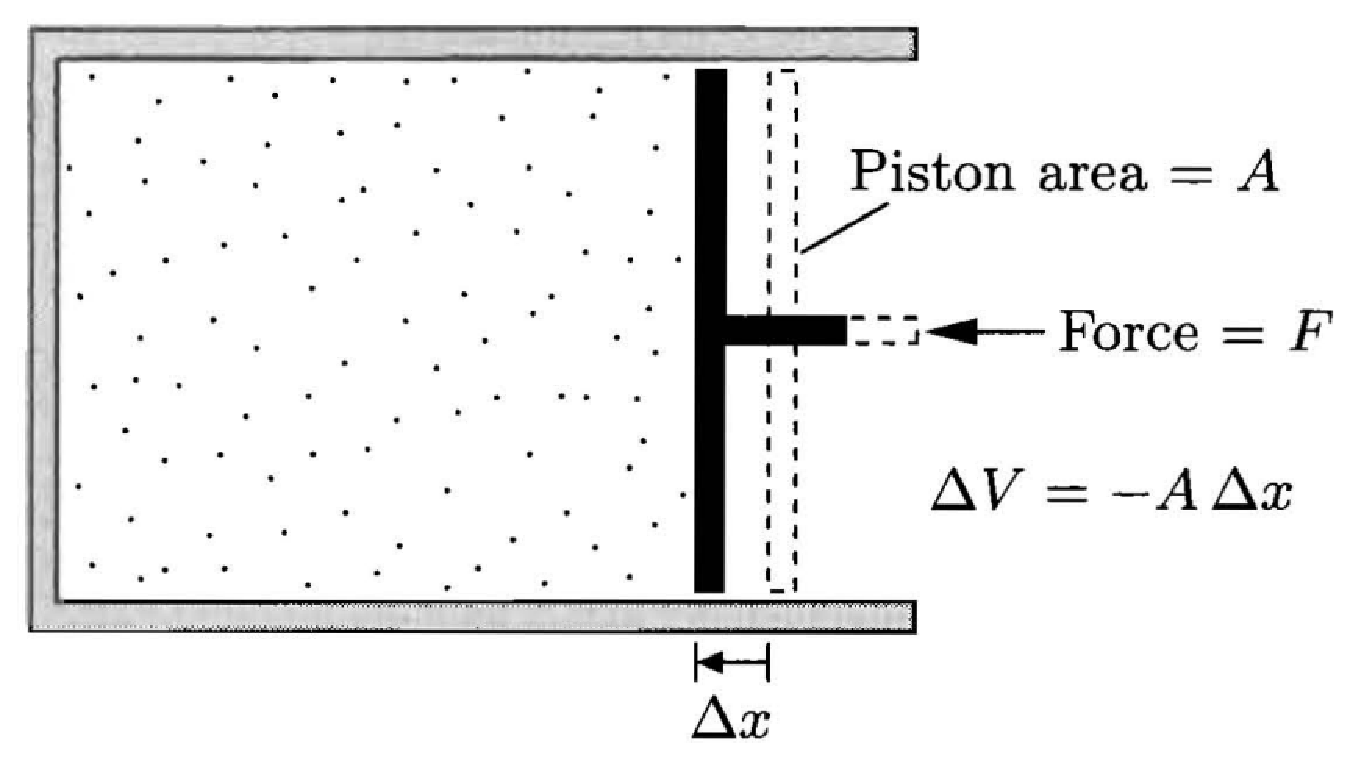
\includegraphics[width=0.7\textwidth]{figs/week05_piston.pdf}
\end{center}

Rearranging the expressions above, we can obtain an expression for the work \textit{put into} the gas by its surroundings (that is, by the external force applied to move the piston).
Still assuming an adiabatic (constant-entropy) process, this input work must match the increase in the gas's average internal energy,
\begin{align*}
  W & = \De\!\vev{E} = -P \De V & & \mbox{for constant entropy.}
\end{align*}
If the entropy is allowed to change, this relation between pressure and work will still hold---as we will see in the next section, we will simply no longer be able to identify the work as the total change in the average internal energy:
\begin{align}
  \label{eq:work_constP}
  W & = -P \De V & & \mbox{more generally.}
\end{align}
Later we will be interested in using the gas as a thermodynamic engine that \textit{does work on} its surroundings.
This removes energy from the gas, corresponding to a negative $W < 0$, and we will need to be careful to keep track of the negative signs and their meaning.

Of course, as we change the volume of the gas, the pressure itself will change as described by the gas's equation of state---such as the ideal gas law, \eq{eq:ideal_gas_law}.
With the equation of state providing an expression $P(V)$ for the pressure as a function of the volume, \eq{eq:work_constP} generalizes to
\begin{equation}
  \label{eq:work}
  W = -\int_{V_0}^{V_f} P(V) \; dV.
\end{equation}
% ------------------------------------------------------------------



% ------------------------------------------------------------------
\subsection{Heat and entropy}
Now let's switch things up by changing the temperature $T$ of an ideal gas while keeping its volume constant.
(As always for the canonical ensemble, the number of particles $N$ is also constant.)
Since the volume is constant, \eq{eq:work} indicates that no work is done, $W = 0$.
Even so, from \eq{eq:ideal_energy} we have $\vev{E} = \frac{3}{2} NT$ and can see that the average internal energy still changes,
\begin{equation}
  \label{eq:dE_dT}
  d\!\vev{E} = \frac{3}{2} N dT.
\end{equation}

In order to remain consistent with our discussion in the previous section, we should expect a change in the entropy to accompany this change in the internal energy that occurs with no work done.
Indeed, for both cases of distinguishable and indistinguishable particles, the temperature dependence of the entropy in \eq{eq:ideal_entropy} is the same:
\begin{equation*}
  S = N\log\left(\lath^{-3}\right) + T\mbox{-independent} = N\log\left(T^{3 / 2}\right) + T\mbox{-independent}.
\end{equation*}
What is the change in the entropy that results from changing the temperature by $dT$?
\begin{mdframed}
  $\displaystyle dS = $ \\[60 pt]
\end{mdframed}
Looking back to \eq{eq:dE_dT}, you should find $d\!\vev{E} = T dS$, which leads us to another important definition.

\begin{shaded}
  The \textbf{heat} added to or removed from a statistical system is defined to be
  \begin{equation}
    \label{eq:heat_def}
    Q = T dS,
  \end{equation}
  and corresponds to the change in the average internal energy of the system when the volume and particle number are kept constant.
\end{shaded}

Just as for the work $W$ considered in previous section, the heat $Q$ is positive when energy is added to the system to increase $\vev{E}$, and negative when energy is removed.
We are used to seeing the entropy as a derived function of the temperature, $S(T)$.
We can generally invert this relation to integrate over the infinitesimal\footnote{Sometimes infinitesimal heat and work are written $dQ$ and $dW$, but this invites misinterpretation as a `change' in heat or work, while the heat and work themselves are already changes in the internal energy.} definition in \eq{eq:heat_def},
\begin{equation}
  \label{eq:heat}
  Q = \int_{S_0}^{S_f} T(S) \; dS,
\end{equation}
with $Q = \De\!\vev{E}$ when the volume is constant.

This relation between heat exchange and changes in the entropy provides useful insight into what it means, physically, for a process to be adiabatic.
In order to keep the entropy constant, an adiabatic process has to occur with no heat moving into or out of the system.
In other words, \textbf{adiabatic processes are fast} enough that the system does not have time to exchange heat with its surroundings 
The opposite extreme would be a process slow enough that any and all possible heat exchange can be completed while it is underway.
Based on our work in \secref{sec:heat_ex}, we can see that such heat exchange will keep the system's temperature equal to the temperature of its surroundings.
Taking that surrounding temperature to be constant, we reach the conclusion that \textbf{constant-temperature (or isothermal) processes are slow}.
Most real processes exist in between these two extremes, usually closer to the adiabatic limit.
% ------------------------------------------------------------------



% ------------------------------------------------------------------
\subsection{Thermodynamic cycles}
Now we can generalize our work in the previous two sections to consider simultaneous changes in the temperature $T$ and the volume $V$ of the gas (still with fixed particle number $N$).
We are used to working with the internal energy $\vev{E}\!(T, V)$ and entropy $S(T, V)$ as functions of the temperature and volume.
Inverting these relations allows us to instead express the temperature $T(S, V)$ and therefore the internal energy as functions of the entropy and volume,
\begin{equation*}
  \vev{E}\!(T, V) \to \vev{E}\!(S, V).
\end{equation*}
Expanding the internal energy to first order in a multi-variable Taylor expansion, we have
\begin{equation*}
  \vev{E}\!(S, V) \approx \vev{E}\!(S_0, V_0) + (S - S_0) \left.\pderiv{\vev{E}}{S}\right|_V + (V - V_0) \left.\pderiv{\vev{E}}{V}\right|_S.
\end{equation*}
This approximation becomes exact in the limit of infinitesimal changes, $(S - S_0) \to dS$, $(V - V_0) \to dV$ and $\vev{E}\!(S, V) - \vev{E}\!(S_0, V_0) \to d\!\vev{E}$.
At the same time, we can recognize the temperature from \eq{eq:temperature} and the (negative) pressure from \eq{eq:pressure}, to obtain
\begin{equation}
  \label{eq:first_law}
  d\!\vev{E} = T dS - P dV = Q + W.
\end{equation}
This is the general form of the \textbf{first law of thermodynamics}: Any change in the internal energy of a statistical system must be matched by (either or both) heat exchange with its surroundings or work done by or on those surroundings.

\begin{shaded}
  We now have all the concepts and \textbf{key equations} needed to consider a variety of ways to manipulate an ideal gas in a container: \\[-24 pt]
  \begin{itemize}
    \item \eq{eq:ideal_energy} for the internal energy $\vev{E} = \frac{3}{2} NT$
    \item \eq{eq:ideal_entropy} for the condition of constant entropy, $V T^{3/2} = \mbox{constant}$
    \item \eq{eq:ideal_gas_law} for the equation of state (ideal gas law): $PV = NT$
    \item \eq{eq:first_law} for the first law of thermodynamics, $d\!\vev{E} = T dS - P dV = Q + W$
  \end{itemize}
\end{shaded}

As examples of manipulations we could carry out just by changing the system's control parameters, the piston shown in the figure above allows us to compress or expand the gas.
This change in volume can be either fast enough to keep the entropy constant (adiabatic) or slow enough to keep the temperature constant (isothermal).
Alternately, we can clamp the piston in place to keep the volume constant, and add heat to the gas to increase its temperature---which will also increase its pressure according to the ideal gas law.
Or we can add heat while keeping the pressure constant by applying a constant force to the piston.
The ideal gas law then implies the volume will increase, pushing out the piston and potentially doing work on the external world.

It's possible to carry out a sequence of such manipulations that cause the system to end up in the same thermodynamic (macro-)state in which it started, with the same pressure, volume, temperature and internal energy.
That sequence can then be repeated over and over again, always ending up back at its starting point.
Such a repeatable process is known as a \textbf{thermodynamic cycle}.
As we will see in the next section, such cycles can make use of heat to have the system do work on its surroundings (providing an \textit{engine}), or make use of work to remove heat from the system (providing a \textit{refrigerator}), among other applications.

Thanks to the key equations above, we can see that the full ideal gas macro-state can be specified solely in terms of the pressure $P$ and the volume $V$.
With fixed $N$, the ideal gas law fixes the temperature $T = \frac{PV}{N}$, which then provides the internal energy $\vev{E} \propto NT$.
It is therefore convenient to represent the system's macro-state in the form of a \textbf{pressure--volume} (or $\mathbf{PV}$) \textbf{diagram}---a plot with the volume on the horizontal axis and the pressure on the vertical axis.
The manipulations discussed above correspond to lines in $PV$~diagrams.
In the case of a thermodynamic cycle, the lines must meet up to form a closed path for the system to go around as the cycle is repeated.

As a first example, the figure below shows the $PV$~diagram for a (slow) isothermal expansion of the gas.
\begin{center}
  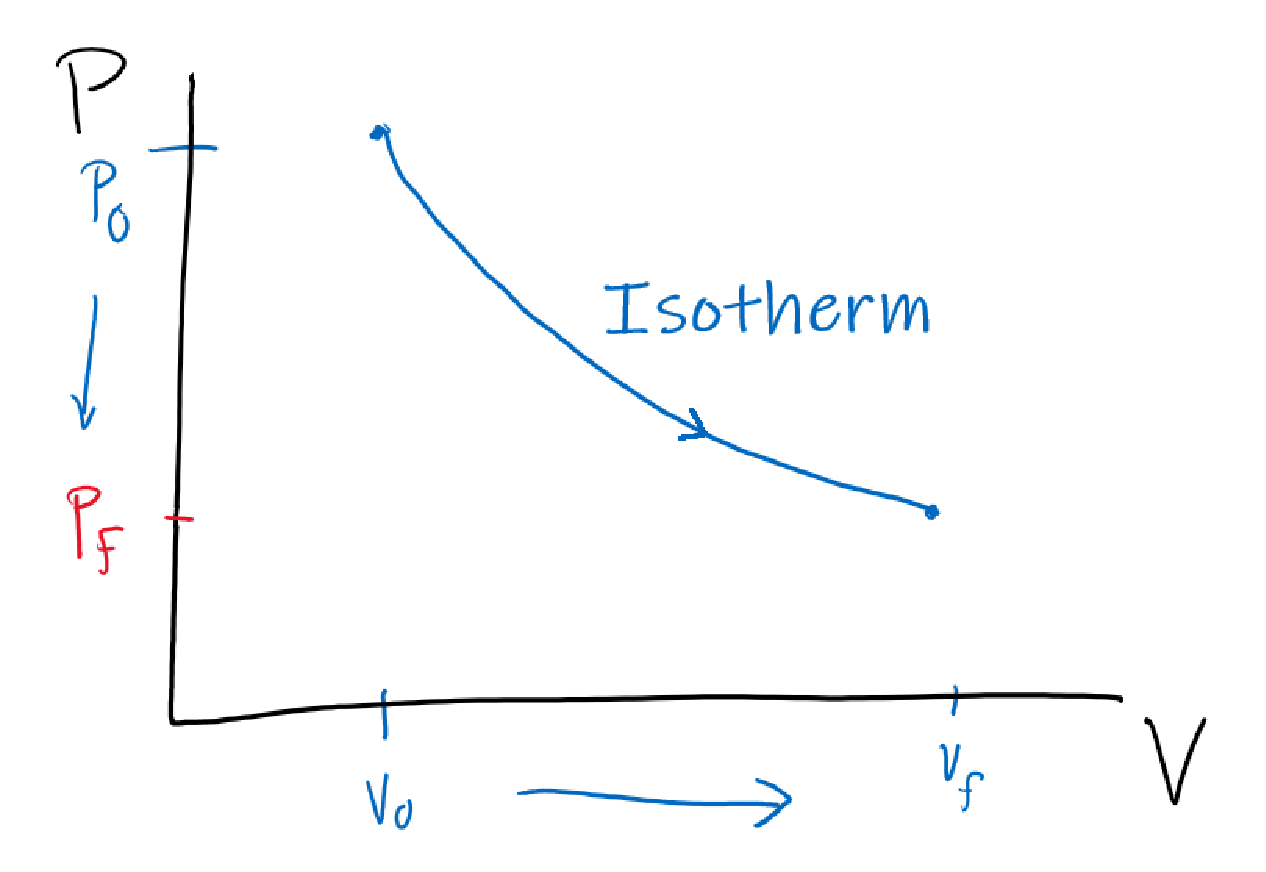
\includegraphics[width=0.6\textwidth]{figs/week05_isotherm.pdf}
\end{center}
\newpage % WARNING: FORMATTING BY HAND
\noindent The line in a $PV$~diagram for an isothermal process is known as an \textit{isotherm}.
As the volume expands from $V_0$ to $V_f$, the temperature (and therefore $PV$) is constant.
What is the change in pressure $\De P = P_f - P_i$ in terms of $P_0$, $V_0$ and $V_f$?
Can isotherms ever cross?
\begin{mdframed}
  \ \\[100 pt]
\end{mdframed}

Similarly, we can consider the $PV$~diagram below for a (fast) adiabatic compression of the gas.
\begin{center}
  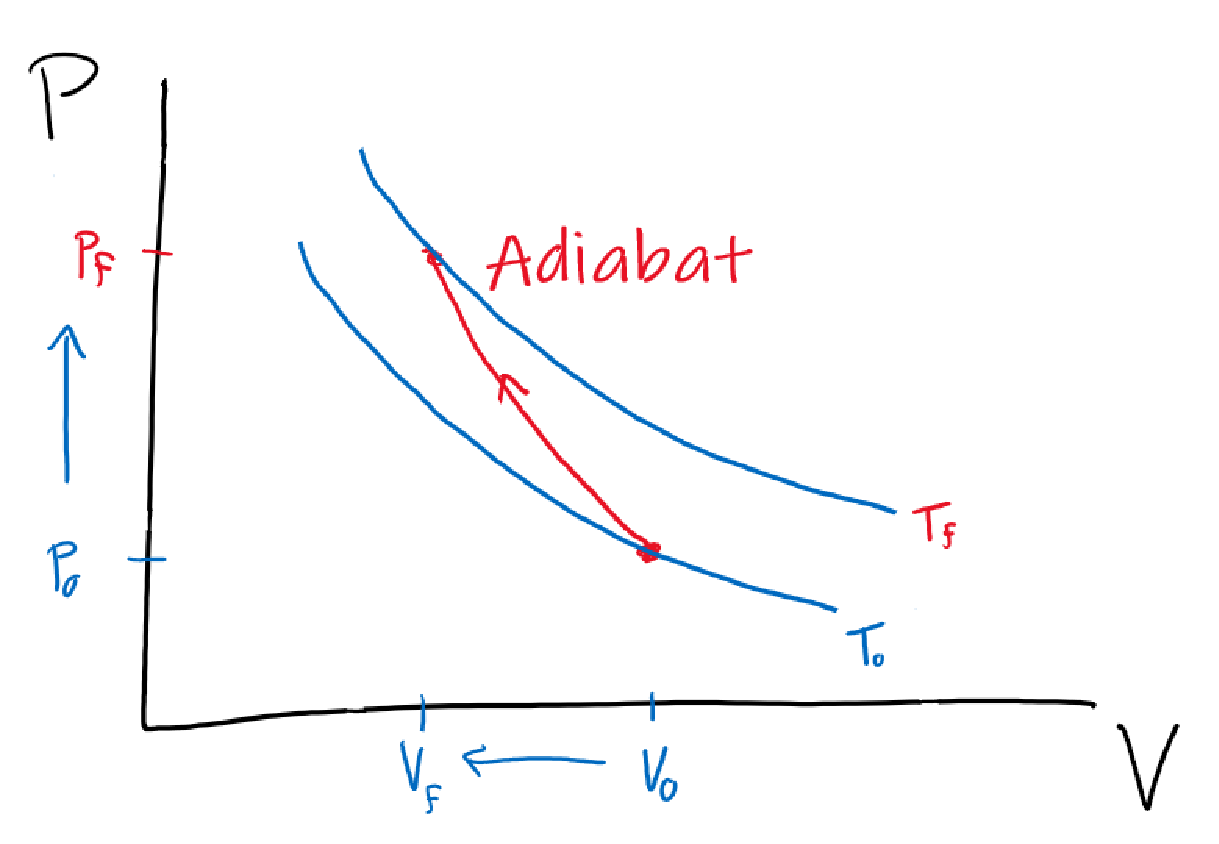
\includegraphics[width=0.6\textwidth]{figs/week05_adiabat.pdf}
\end{center}
In this case both the pressure and temperature change, while the entropy (and therefore $VT^{3 / 2}$) is constant.
What are $\De P$ and the change in the temperature $\De T = T_f - T_0$ in terms of $P_0$, $V_0$, $V_f$ and the fixed number of particles $N$?
\begin{mdframed}
  \ \\[120 pt]
\end{mdframed}
% ------------------------------------------------------------------



% ------------------------------------------------------------------
\subsection{The Carnot cycle}
A famous thermodynamic cycle was proposed by \href{https://en.wikipedia.org/wiki/Nicolas_Léonard_Sadi_Carnot}{Sadi Carnot} in 1824, and laid the groundwork for subsequent development of engines and refrigerators later in the nineteenth century.
The key idea is to propose that the ideal gas's container can exchange energy with either of two different thermal reservoirs: a `hot' reservoir with temperature $T_H$ and a `cold' reservoir with temperature $T_L$.
The Carnot cycle consists of four stages, which are first shown below in the form of a $PV$~diagram, then illustrated in a sketch (adapted from Schroeder's \textit{Introduction to Thermal Physics}) that provides a more concrete picture of the physical processes, and finally summarized in words.

\begin{center}
  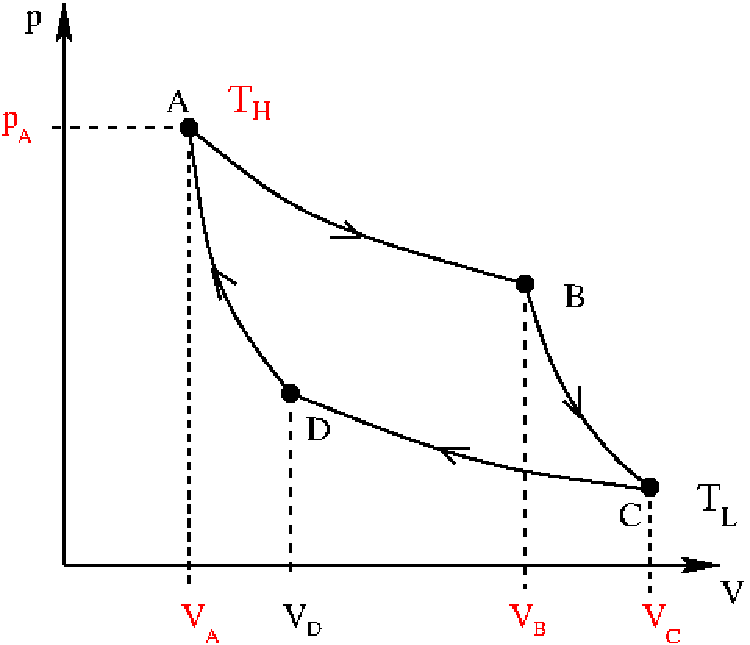
\includegraphics[width=0.6\textwidth]{figs/week05_carnot-PV.pdf} \\[36 pt]
  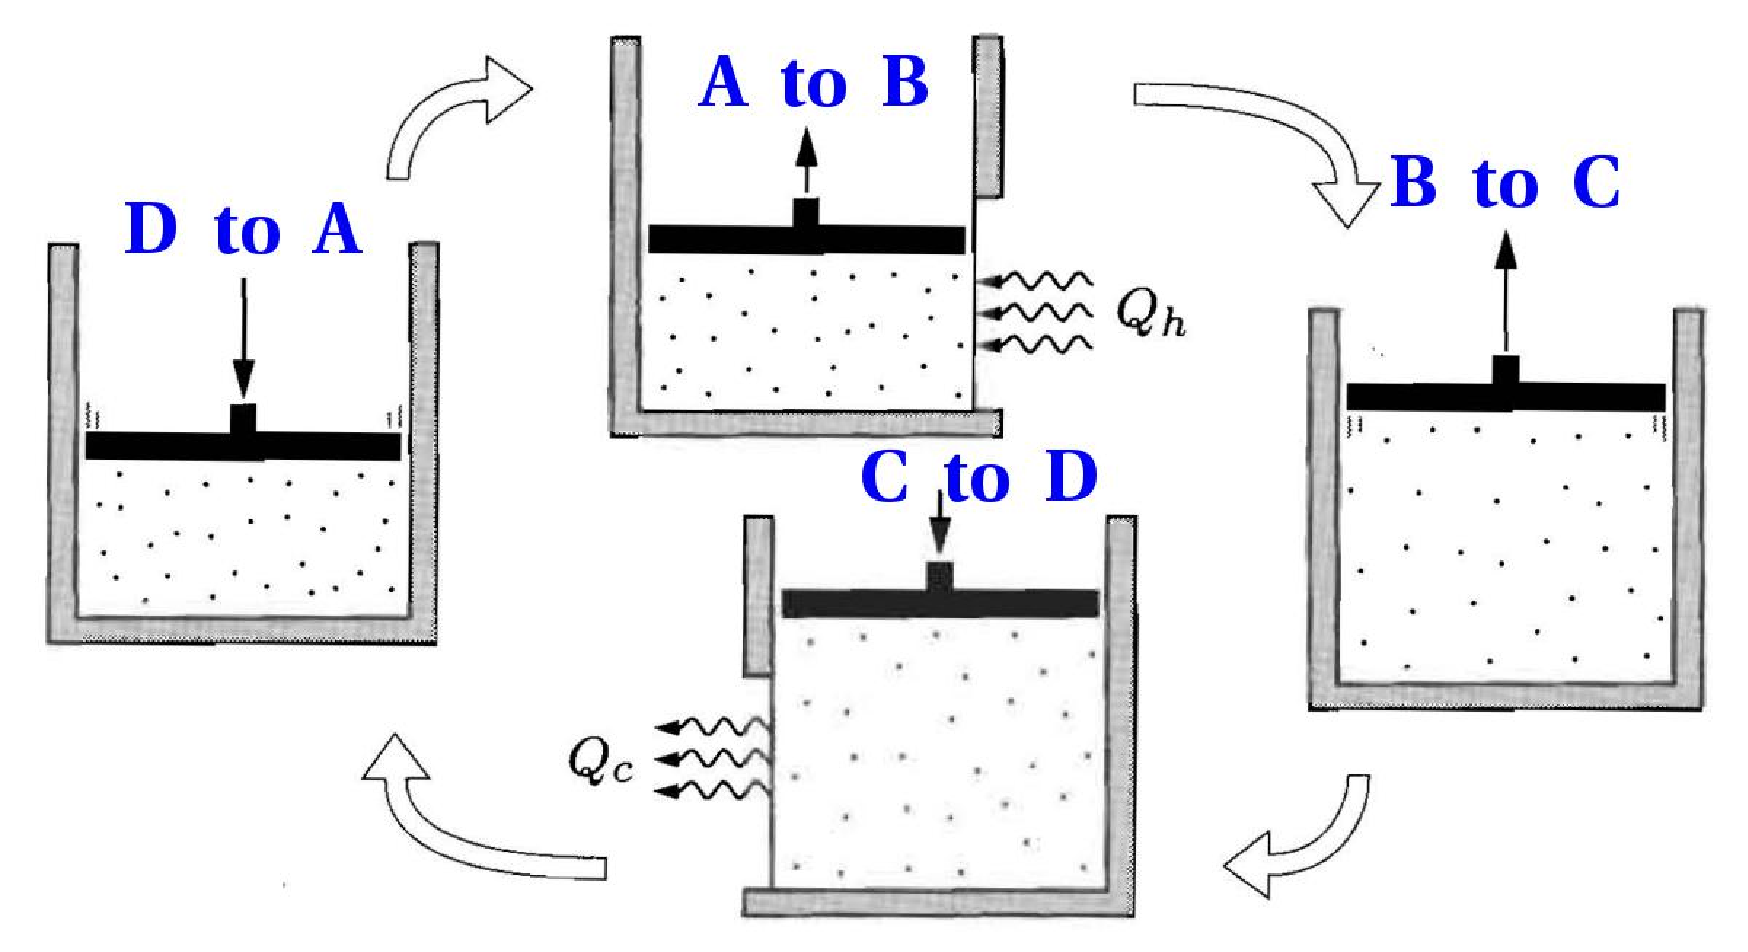
\includegraphics[width=\textwidth]{figs/week05_carnot.pdf}
\end{center}

\newpage % WARNING: FORMATTING BY HAND
The illustration above supposes that the hot reservoir is located to the right of the system, while the cold reservoir is located to its left.
In words, the four stages are the following: \\[-24 pt]
\begin{itemize}
  \item From point $A$ to point $B$ the system undergoes slow isothermal expansion, bringing in heat $Q_{\text{in}}$ from the hot reservoir in order to keep its temperature fixed at $T_H$.
  \item From point $B$ to point $C$ the system undergoes fast adiabatic expansion, with no heat exchange, until its temperature falls from $T_H$ down to $T_L$.
  \item From point $C$ to point $D$ the system undergoes slow isothermal compression, expelling heat $Q_{\text{out}}$ into the cold reservoir in order to keep its temperature fixed at $T_L$.
  \item From point $D$ to point $A$ the system undergoes fast adiabatic compression, with no heat exchange, until its temperature rises from $T_L$ back up to $T_H$.
\end{itemize}

We need to make sure that these four processes really do produce a closed, self-consistent cycle that our system could repeatedly follow.
In a real experiment, we would have full control over the four variables $\left\{P_A, V_A, V_B, V_C\right\}$ coloured red in the $PV$~diagram above.
Specifically, we can prepare our $N$-particle system in initial macro-state $A$ with our choice of pressure $P_A$ and volume $V_A$, which together fix the temperature $T_H = \frac{P_A V_A}{N}$ through the ideal gas law.
We can then choose how much isothermal expansion occurs to reach volume $V_B$, and finally choose how much adiabatic expansion occurs to reach volume $V_C$.
The question then becomes: Is it possible to return to our starting macro-state $A$ by choosing the appropriate volume $V_D$ at which to switch from isothermal compression to adiabatic compression?

To answer this question, we should try to express all the remaining variables $\left\{P_B, P_C, T_L, P_D, V_D\right\}$ in terms of the four (red) inputs described above, along with the fixed number of particles $N$.
At point $B$, we know the system's temperature remains $T_H = P_A V_A / N$.
What is the pressure $P_B$ in terms of $\left\{P_A, V_A, V_B, V_C, N\right\}$?
\begin{mdframed}
  \ \\[50 pt]
\end{mdframed}

\newpage % WARNING: FORMATTING BY HAND
At point $C$, we know the system's entropy is the same as at point $B$.
What are the temperature $T_L$ and pressure $P_C$ in terms of $\left\{P_A, V_A, V_B, V_C, N\right\}$?
\begin{mdframed}
  \ \\[100 pt]
\end{mdframed}

At point $D$, we know the system's temperature remains $T_L$, and demand that its entropy is the same as at point $A$.
What are the pressure $P_D$ and volume $V_D$ in terms of $\left\{P_A, V_A, V_B, V_C, N\right\}$?
\begin{mdframed}
  \ \\[100 pt]
\end{mdframed}

You should find that all of $\left\{P_B, P_C, T_L, P_D, V_D\right\}$ can be consistently specified by the (red) inputs under our control, which establishes that the Carnot cycle is a valid thermodynamic cycle.
Now we can consider the more interesting question of how much work (if any) this cycle can do on its surroundings, compared to the amount of heat it would need to operate.
It will simplify this calculation to use the following positive quantities, with subscripts (rather than negative signs) indicating whether energy is flowing into or out of the gas: \\[-24 pt]
\begin{itemize}
  \item When work is done on the system by its surroundings, $W_{\text{in}} = W > 0$ from \eq{eq:work}
  \item When work is done by the system on its surroundings, $W_{\text{out}} = -W > 0$
  \item When heat enters the system, $Q_{\text{in}} = Q > 0$ from \eq{eq:heat_def}
  \item When heat leaves the system, $Q_{\text{out}} = -Q > 0$
\end{itemize}
We can now define a convenient combination of heat and work to consider.

\begin{shaded}
  The \textbf{efficiency} $\eta$ of a thermodynamic engine is defined to be
  \begin{equation}
    \label{eq:efficiency}
    \eta = \frac{W_{\text{done}}}{Q_{\text{in}}} = \frac{W_{\text{out}} - W_{\text{in}}}{Q_{\text{in}}},
  \end{equation}
  where $W_{\text{done}} = W_{\text{out}} - W_{\text{in}}$ is the \textit{net} amount of work done by each repetition of the cycle, while $Q_{\text{in}}$ is the \textit{total} amount of heat that enters the system in each repetition.
\end{shaded}

By specifying a thermodynamic \textit{engine}, we assume $W_{\text{out}} > W_{\text{in}}$, so that the overall cycle does more work on its surroundings than it requires as input to operate.
This corresponds to $\eta > 0$, and we can also put an upper bound on the efficiency, due to the first law of thermodynamics, \eq{eq:first_law}.
Because the system returns to its initial macro-state after each repetition of the cycle, we have
\begin{align}
  \De\!\vev{E} = 0 & = Q_{\text{in}} - Q_{\text{out}} + W_{\text{in}} - W_{\text{out}} \cr
                   & \Lra W_{\text{out}} - W_{\text{in}} = Q_{\text{in}} - Q_{\text{out}} \leq Q_{\text{in}}, \label{eq:cycle_heat_work}
\end{align}
or $\eta \leq 1$, with equality occurring when no waste heat is expelled throughout the entire cycle, $Q_{\text{out}} = 0$.
All together, $0 < \eta \leq 1$ lets us interpret the efficiency as the fraction of the input heat that the engine is able to use to do work on its surroundings.

Let's illustrate these ideas by computing the efficiency of the Carnot cycle.
We can divide this task into smaller pieces by considering the contributions to $W_{\text{done}}$ and $Q_{\text{in}}$ from each of the cycle's four stages.
First, in the isothermal expansion from point $A$ to point $B$, the ideal gas law provides $P(V)$ to insert into \eq{eq:work}:
\begin{mdframed}
  $\displaystyle W_{AB} = -\int_{V_A}^{V_B} P(V) \; dV = $ \\[50 pt]
\end{mdframed}
You should find $W_{AB} < 0$, meaning the system does work on its surroundings during this stage.
At the same time, the constant temperature means $\De\!\vev{E} \propto \De T = 0$ from \eq{eq:ideal_energy}, so that $Q_{AB} = -W_{AB} > 0$ and heat flows into the system.

\newpage % WARNING: FORMATTING BY HAND
Next, in the adiabatic expansion from point $B$ to point $C$, we know $Q_{BC} = 0$ and therefore
\begin{mdframed}
  $\displaystyle W_{BC} = \De\!\vev{E} = \frac{3}{2}N\De T = $ \\[50 pt]
\end{mdframed}
You should find that the system continues doing work on its surroundings during this stage, $W_{BC} < 0$.

Finally, the computations for the two compression stages are directly analogous to those above.
For the isothermal compression from point $C$ to point $D$, we have
\begin{mdframed}
  $\displaystyle W_{CD} = -\int_{V_C}^{V_D} P(V) \; dV = $ \\[50 pt]
\end{mdframed}
Now you should find $W_{CD} > 0$, meaning this compressions requires work to be done on the system by its surroundings, while $Q_{CD} = -W_{CD} < 0$ means heat flows out of the system.
For the adiabatic compression from point $D$ to point $A$, we know $Q_{DA} = 0$ while the change in temperature is exactly opposite the $\De T$ of the $B \to C$ adiabatic expansion.
Therefore $W_{DA} = -W_{BC} > 0$ and more work has to be done on the system to complete the cycle.

Putting everything together,
\begin{align}
  W_{\text{out}} & = -W_{AB} - W_{BC} \cr
  W_{\text{in}} & = W_{CD} + W_{DA} = W_{CD} - W_{BC} \cr
  Q_{\text{in}} & = Q_{AB} = -W_{AB} \cr
  \eta & = \frac{-W_{AB} - W_{BC} - W_{CD} + W_{BC}}{-W_{AB}} = 1 + \frac{W_{CD}}{W_{AB}} = 1 - \frac{T_L}{T_H}.
\end{align}
We can check that our result $\eta = 1 - \frac{T_L}{T_H}$ for the efficiency of the Carnot cycle makes sense.
Since $T_L < T_H$, we have $\eta > 0$.
If the temperatures of the hot and cold reservoirs approached each other, $\frac{T_L}{T_H} \to 1$, then there would no longer be any heat exchange, and the engine would cease to function, with its efficiency $\eta \to 0$.
In the opposite limit of a large difference in the temperatures $T_L \ll T_H$, the efficiency would improve, with $\eta \to 1$ as $\frac{T_L}{T_H} \to 0$.

It turns out to be generic for heat engines to operate more efficiently as the temperature difference between their hot and cold reservoirs increases, and they always cease working as $\frac{T_L}{T_H} \to 1$.
The Carnot cycle is special because its efficiency $\eta = 1 - \frac{T_L}{T_H}$ is the theoretical maximum allowed by the second law of thermodynamics.
We can show this by using \eq{eq:cycle_heat_work} to rewrite
\begin{equation*}
  \eta = \frac{Q_{\text{in}} - Q_{\text{out}}}{Q_{\text{in}}} = 1 - \frac{Q_{\text{out}}}{Q_{\text{in}}} = 1 - \frac{T_L \De S_{\text{out}}}{T_H \De S_{\text{in}}},
\end{equation*}
where the last equality uses \eq{eq:heat} and the generic fact that the input heat $Q_{\text{in}} = T_H \De S_{\text{in}}$ enters the engine from the hot reservoir while the waste heat $Q_{\text{out}} = T_L \De S_{\text{out}}$ is expelled to the cold reservoir.
After each repetition of the cycle, the gas returns to its original macro-state, with its original entropy, after absorbing entropy $\De S_{\text{in}}$ from its surroundings and expelling $\De S_{\text{out}}$ back out again.
The second law therefore demands $\De S_{\text{out}} \geq \De S_{\text{in}}$, so that
\begin{equation*}
  \eta = 1 - \frac{T_L}{T_H} \frac{\De S_{\text{out}}}{\De S_{\text{in}}} \leq 1 - \frac{T_L}{T_H}
\end{equation*}
in principle, for any thermodynamic engine.

Finally, if we were to operate the Carnot cycle in reverse, with isothermal expansion at temperature $T_L$ and compression at $T_H$, we would do work on the system in order to bring heat in from the cold reservoir and expel it to the hot reservoir.
In other words, we would have a refrigerator rather than an engine.
The `efficiency' of a refrigerator is called its \textit{coefficient of performance}, and defined as
\begin{equation*}
  \mathrm{COP} = \frac{Q_{\text{in}}}{W_{\text{in}} - W_{\text{out}}} = \frac{Q_{\text{in}}}{Q_{\text{out}} - Q_{\text{in}}} = \frac{1}{Q_{\text{out}} / Q_{\text{in}} - 1} \leq \frac{1}{T_H / T_L - 1} = \frac{T_L}{T_H - T_L},
\end{equation*}
which can be greater than one.
The reversed Carnot cycle provides the best possible $\mathrm{COP}$ for a refrigerator.
Despite its efficiency, the Carnot cycle does not provide a practical engine or refrigerator, simply because its slow isothermal stages take too long!
Real engines and refrigerators sacrifice efficiency for functionality.
% ------------------------------------------------------------------
